\documentclass[preview]{standalone}

\usepackage{amsmath}
\usepackage{amssymb}
\usepackage{stellar}
\usepackage{bettelini}
\usepackage{soul}

\hypersetup{
    colorlinks=true,
    linkcolor=black,
    urlcolor=blue,
    pdftitle={Stellar},
    pdfpagemode=FullScreen,
}

\begin{document}

\title{Stellar}
\id{italiano-oltre-la-spera}
\genpage

\section{Testo}

\plain{Il seguente sonetto descrive il concetto di <b>intelligenza nova</b>
indotta nello spirito di Dante.}

\begin{snippet}{oltre-la-spera-1-4}
    \StellarPoetry{1}{
        Oltre la spera che più larga gira, \\
        passa 'l sospiro ch'esce del mio core: \\
        intelligenza nova, che l'Amore \\
        piangendo mette in lui, pur sù lo tira. 
    }{
        Al di là del cielo che ruota più largamente
        passa il pensiero ('l sospiro) che esce dal mio cuore: 
        una nuova capacità di comprendere (intelligenza nova), che l'Amore
        mette in lui tra le lacrime (piangendo), lo solleva di continuo in alto (pur su lo tira).
    }

    Il primo verso è una perifrasi che indica \quotes{oltre il pianeta più lontano} (chiamato \textit{Il Primo Nobile}), ossia il paradiso
    siccome la visione dell'universo era quella tolemaica e creazionista.
    
    Il secondo verso ci indica che il sospiro del poeta esce dal suo cuore, mentre è vivo, dalla sua intimità più profonda,
    e attraverso i cieli fino al paradiso.  
    
    Ai versi 3-4 viene descritto ciò che permette questo percorso, ossia ciò che lo tira
    verso l'alto. Questa forza è un'intelligenza nova, ossia una nuova sensibilità nel vedere le cose.
    Questa nuova intelligenza deriva dall'amore, che permette all'autore di avere una nuova consapevolezza.
    Questa esperienza amorosa è dolorosa ma porta ad una nuova capacità di intendimento.
    Inoltre, la parola amore ha la maiuscola perché esso viene personificato.
\end{snippet}

\begin{snippet}{oltre-la-spera-5-8}
    \StellarPoetry{5}{
        Quand'elli è giunto là dove disira, \\
        \textbf{vede} una donna, che riceve onore, \\
        e \textbf{luce} sì, che per lo suo \textbf{splendore} \\
        lo peregrino spirito la \textbf{mira}.
    }{
        Quando esso [il sospiro] è arrivato là dove desidera [nell'Empireo],
        vede una donna che viene onorata e risplende (luce) a tal punto che lo
        spirito pellegrino la ammira per il suo splendore.
    }

    La seconda quartina descrive il punto di arrivo.
    Quando lo spirito arriva, vede una donna, la quale viene onorata dagli altri beati, Dio e la Madonna.
    Viene anche detto che questa donna brilla.
    A causa di questo grande splendore, lo spirito giunto in paradiso (pellegrino, in pellegrinaggio) la ammira.
\end{snippet}

\begin{snippet}{oltre-la-spera-9-11}
    \StellarPoetry{9}{
        \textbf{Vedela} tal, che quando 'l mi ridice, \\
        io no lo \textbf{'ntendo}, sì \textbf{parla} sottile \\
        al cor dolente, che lo fa \textbf{parlare}.
    }{
        [Il sospiro] la vede in tal modo (Vedela tal), che quando tenta di descrivermela
        ('l mi ridice) io non lo capisco (no lo intendo), a tal punto
        (sì) parla in modo complesso (sottile) al cuore addolorato che lo spinge a raccontare.
    }

    Lo spirito ripercorre il medesimo tragitto verticale, ma al contrario, tornando da Dante.
    Questo spirito cerca di spiegargli che cosa ha visto.
    \quotes{La vede tale che quando me lo ridice, io non capisco}.
    Dante non comprende quindi ciò che lo spirito gli riferisce, perché
    \quotes{parla sottile}, ossia parla in maniera troppo difficile.
    Il cuore dolente del poeta è ciò lo fa sì che lo spirito venga interrogato.
    Infatti, lo spirito parla proprio al cuore \underline{e} a Dante (questo amplifica l'incomprensione della spiegazione).
    Lo spirito parla in maniera troppo complessa perché il linguaggio non riesce
    ad esprimere quello che si è provato (topos dell'ineffabilità, è ineffabile)
    siccome l'esperienza lo tracende.
\end{snippet}

\begin{snippet}{oltre-la-spera-12-14}
    \StellarPoetry{12}{
        So io che \textbf{parla} di quella gentile, \\
        però che spesso \textbf{ricorda} Beatrice, \\
        \st{sì ch'io lo \textbf{'ntendo} ben, donne mie care.}
    }{
        Io so che parla di quella nobildonna (gentile) dal
        momento che (però che) cita (ricorda) spesso il nome
        di Beatrice, cosicché io lo capisco bene [che sta parlando di Beatrice], mie care donne.
    }

    \textbf{\color{red}Nota:} La parola \quotes{però} significa \quotes{per ciò}. \\
    Questa è l'unica occorrenza dove Beatrice viene nominata direttamente in un testo poetico in \textit{Vita Nova}.\\
    Nell'incomprensione fra Dante e lo spirito, Dante capisce che la donna vista era sicuramente
    Beatrice. \\
    Nella poesia antica, la parola \textit{gentile} è molto più profonda di quella odierna
    e possiede un significato diverso. Essa ha un significato nobile di purezza (nobiltà d'animo).
    
    L'ultimo verso è dato dal fatto che Dante si stesse riferendo a delle Donne nel testo.
\end{snippet}

\section{Analisi}

\begin{snippet}{oltre-la-spera-analisi}
    Questo sonetto è diviso in due parti, dove vengono distinte le due verticalità del viaggio dello spirito
    (avanti e indietro).
    
    Molte parole della prima parte appartendono alla sfera visiva, poiché il paradiso
    è fatto di luci, mentre molte parole della seconda fanno parte del parlare.
    Questo è dato dal fatto che lo spirito può vedere, ma ha l'impossibilità di esprimersi.
    
    Questa separazione è collegata dall'uso di due parole quasi uguali,
    \textbf{mira} e \textbf{Vedela} (detto per anadiplosi).
\end{snippet}

% TODO atoni e tonici

\begin{snippetdefinition}{legge-tobler-mussafia-definition}{Legge di Tobler Mussafia}
    È vietato iniziare un verso (poesie o prosa) o far seguire una congiunzione coordinante
    con un pronome atoni.
\end{snippetdefinition}

\begin{snippet}{asdasd}
    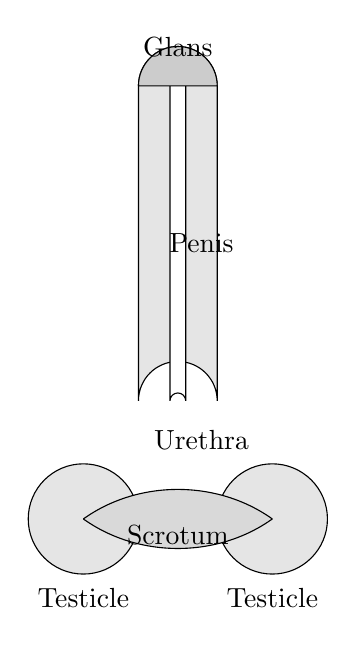
\begin{tikzpicture}
        % Penis
        \draw[fill=gray!20] (2,0) -- (2,4) arc[start angle=180, end angle=0, radius=0.5] -- (3,0) arc[start angle=0, end angle=180, radius=0.5];
        
        % Urethra
        \draw[fill=white] (2.4,0) -- (2.4,4) arc[start angle=180, end angle=0, radius=0.1] -- (2.6,0) arc[start angle=0, end angle=180, radius=0.1];
    
        % Glans
        \draw[fill=gray!40] (2,4) arc[start angle=180, end angle=0, radius=0.5] -- (3,4) -- (2,4);
    
        % Testicles
        \draw[fill=gray!20] (1.3,-1.5) circle (0.7);
        \draw[fill=gray!20] (3.7,-1.5) circle (0.7);
        
        % Scrotum
        \draw[fill=gray!30] (1.3,-1.5) .. controls (2,-2) and (3,-2) .. (3.7,-1.5);
        \draw[fill=gray!30] (1.3,-1.5) .. controls (2,-1) and (3,-1) .. (3.7,-1.5);
    
        % Labels
        \node at (2.5, 4.5) {Glans};
        \node at (2.8, 2) {Penis};
        \node at (2.8, -0.5) {Urethra};
        \node at (1.3, -2.5) {Testicle};
        \node at (3.7, -2.5) {Testicle};
        \node at (2.5, -1.7) {Scrotum};
    \end{tikzpicture}
\end{snippet}

\end{document}